\documentclass[10pt]{beamer}
\usetheme{hsrm}
\usepackage[utf8]{inputenc}
\usepackage[spanish]{babel}
\usepackage{amsmath}
\usepackage{xcolor}
%\usecolortheme{spruce}
\usepackage{here}
\graphicspath{{./Images/}}
\usepackage{verbatim}
\usepackage{amsfonts}
\usepackage{marvosym}
\usepackage[marvosym]{tikzsymbols}
\usepackage{tikz}
\usepackage{tikzducks}
\usepackage{amssymb}
\usepackage{graphicx}
\usefonttheme{professionalfonts}
\title{\Large Bringing innovation to market: business models for battery storage}
\subtitle{\tiny Trayendo innovación al mercado: modelos de negocios para el almacenamiento de baterías}
%\author{Josue Huaroto Villavicencio}
%\institute{\today}
\date{Josue Huaroto Villavicencio \\[90pt]\today  \\[10pt] \vskip1ex Universidad Nacional de Ingeniería - Facultad de Ingeniería Mecánica}
%\institute[UNI]{Universidad Nacional de Ingeniería}
\begin{document}
\begin{frame}
%
\includegraphics[scale=0.05]{./Images/logoUNI.png}
\maketitle
\end{frame}
\begin{frame}{Abstract}
\begin{abstract}
Los sistemas de energía en todo el mundo han experimentado transiciones significativas hacia una descentralización y descarbonización con mayores requisitos de seguridad y flexibilidad de suministro. El avance tecnológico ayuda a mejorar la eficiencia energética y reducir los costos, lo que a su vez promueve el crecimiento del almacenamiento de baterías a nivel internacional. Los modelos comerciales de almacenamiento de baterías siguen siendo vagos debido a sus primeras etapas de desarrollo, pero está claro que no existe un modelo comercial universal para las baterías dada la amplitud de las aplicaciones. En este estudio, se revisa los componentes principales de los modelos comerciales existentes y destacamos las áreas que se fortalecerán en un modelo comercial nuevo. Por último, pero no menos importante, es importante considerar las innovaciones en otras tecnologías para el diseño de un modelo de negocio.
\end{abstract}
\end{frame}
\begin{frame}
\frametitle{Introducción}
Las energías renovables han estado creciendo rápidamente; en comparación de los combustibles fósiles, el gas natural o el petróleo diesel usado en las islas, la energía renovable tiene menos impacto ambiental durante su ciclo de vida. Se ha vuelto menos costoso debido a la fabricación, implementación y mejora tecnológica a gran escala. Sin embargo, la integración de energía renovable a gran escala requiere un mayor nivel de flexibilidad en el sistema de energía para permitir nuevas formas de innovación.\\
Hay muchas formas de aumentar la flexibilidad de un sistema de energía. Hoy en día, el almacenamiento de energía se está volviendo cada vez más popular; presenta la solución más prometedora para abordar las variaciones de la producción de energía renovable. Dependiendo de la forma de energía utilizada, existen muchos tipos diferentes de sistemas de almacenamiento de energía. Como una de las tecnologías de almacenamiento más prometedoras, las baterías se han vuelto cada vez más populares en los últimos años. Sin embargo, el modelo de negocio de almacenamiento de baterías sigue siendo impreciso dada su etapa inicial de desarrollo y especificidades de cada aplicación.
\end{frame}
\begin{frame}
\frametitle{Modelo de negocio}
Un modelo de negocio cubre las formas en que la compañía satisface las necesidades del cliente, atrae a los clientes a pagar por su producto o servicio y genera ingresos a partir del pago del cliente. Junto con los modelos de negocio, las empresas emplean estrategias que les permiten posicionarse en el mercado. Además de los costos e ingresos, un modelo de negocio también cubre otros factores como segmentos de clientes, propuestas de valor, canales para llegar a clientes, socios, etc. Osterwalder y Pigneur indican que un modelo de negocio exitoso consta de nueve bloques de construcción, que incluyen segmentos de clientes, propuesta de valor, canales, relaciones con clientes, flujos de ingresos, recursos clave, actividades clave, asociaciones clave y estructura de costos. En otro estudio, Johnson, et al. introduce cuatro componentes principales en un modelo de negocio exitoso: una propuesta de valor para el cliente, una fórmula de ganancias, recursos clave y procesos clave.
\end{frame}
\begin{frame}
\frametitle{Modelos de negocio de almacenamiento de baterías}
Pollitt aborda tres componentes principales en los modelos de negocio de almacenamiento de baterías, incluida la propuesta de valor, la creación de valor y la captura de valor. El almacenamiento de la batería ofrece decenas de servicios. Cada servicio está asociado con un flujo de ingresos. El Instituto Rocky Mountain describe trece servicios que las baterías pueden proporcionar en tres niveles de red: detrás del medidor, distribución y transmisión.\\
En términos de creación de valor, los servicios de almacenamiento de batería pueden proporcionar valor a diferentes partes interesadas. Para las baterías instaladas con una planta de energía renovable, el almacenamiento puede ayudar a cambiar la generación de energía renovable que hace que la planta sea más flexible y es aplicable a pequeña escala comunitaria y grandes sistemas a escala de cuadrícula. Para la captura de valor, depende de los servicios que las baterías brinden a cuadrícula. Es poco probable que el enfoque en la provisión de servicios únicos ofrezca un modelo rentable; por lo tanto, los servicios deben combinarse.
\end{frame}
\begin{frame}
\frametitle{Modelos de negocio de almacenamiento de baterías}
En la evaluación de beneficios, uno de los principales desafíos está en la agregación de beneficios. Estos incluyen conflictos operacionales,
conflictos técnicos, barreras regulatorias y agregación de beneficios de múltiples partes interesadas. Primero, servicios de almacenamiento de batería. Necesita compatibilidad operativa. En otras palabras, la provisión de servicios secundarios no debería tener operaciones
conflictos con la provisión de servicios primarios.
\begin{figure}[H]
\centering
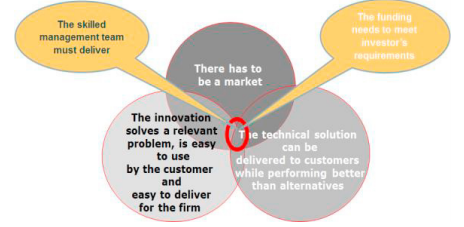
\includegraphics[scale=0.38]{img1.png}
\caption{Cinco factores que determinan el potencial de una innovación}
\end{figure}
\end{frame}
\begin{frame}
\frametitle{Aplicación de baterías existente y su modelo de negocio}
Una de las aplicaciones de los paquetes de baterías de Tesla es la implementación del sistema de baterías de iones de litio de 52 MWh (13MW)
en asociación con Kauai Island Utility Cooperative (KIUC). Las unidades se despliegan cerca de una granja solar que tiene una capacidad de generación total de 13 MW. Según el acuerdo, KIUC acuerda comprar energía del sistema de batería durante 20 años a una tasa de 13,9 centavos por kilovatio-hora, que es más barato que el poder adquisitivo del diesel existente.
En 2017, Tesla también instaló 20 MW de 4 horas sistema de baterías de iones de litio en la subestación Mira Loma de Southern California Edison en Ontario. El sistema de batería se carga durante el día cuando la producción solar alcanza su máximo y libera energía durante los picos nocturnos. El proyecto es parte de una respuesta de emergencia a la posible escasez de energía debido a una gran fuga de gas natural del Alison Canyon, en 2015. De hecho, la fuga de almacenamiento de gas ha impulsado el crecimiento del sistema de almacenamiento de baterías en los últimos años, ya que las empresas de servicios públicos tienen que buscar alternativas en un período de tiempo muy corto para proporcionar seguridad
suministro durante las horas pico. 
\end{frame}
\begin{frame}
\frametitle{Aplicación de baterías existente y su modelo de negocio}
El almacenamiento de la batería en los casos anteriores se utiliza para abordar necesidades específicas en el sistema de energía. Primero, debe haber suficiente producción de energía barata que pueda garantizar la carga de la batería a un costo mínimo. Esta suele ser el caso cuando hay disponibles fuentes de energía renovables a gran escala. Segundo, los costos de usar el  almacenamiento de la batería son más baratos para servicios específicos que cualquier servicio existente. En tercer lugar, existe una necesidad urgente de reemplazar los generadores existentes debido a un cierre inesperado. Entonces, los costos no fueron la principal preocupación en comparación con seguridad. Estos experimentos mejoran gradualmente las aplicaciones de baterías a diferentes escalas en diferentes ubicaciones.\\
Los clientes que también necesitan tener instalado el sistema de techo solar pueden pagar una pequeña tarifa mensual a cambio de un subsidio anual de consumo. La pequeña tarifa mensual reemplaza el cargo por uso convencional y el suministro fijo cargo, que es mucho más bajo que el poder adquisitivo de la red.
\end{frame}
\begin{frame}
\frametitle{Innovación de modelo de negocio}
Aunque el almacenamiento de la batería ha experimentado un rápido crecimiento en los últimos años, su aplicación para el almacenamiento de energía sigue siendo en la etapa inicial de desarrollo y enfrenta varias restricciones. Además de los componentes discutidos anteriormente, un modelo de negocio exitoso debe considerar lo siguiente:
\begin{itemize}
\item Sistema de electricidad en transición.
\item Mercado y barreras regulatorias.
\item La inclusión de externalidades en la evaluación económica.
\item Desarrollo de otras innovaciones.
\end{itemize}
\end{frame}
\begin{frame}
\frametitle{Conclusión}
No es posible abordar un solo modelo de negocio para baterías, ya que una medida única no sirve para todos. Modelos comerciales de baterías
debe distinguirse a diferentes escalas (escala de utilidad vs. aplicación detrás del medidor) que aborde diferentes necesidades
(para reemplazar el sistema existente o agregar un nuevo sistema). Antes de ser competitivos en costos, también deben apuntar a
ubicaciones con diferentes requisitos de energía. Un modelo de negocio exitoso de un sistema de almacenamiento de batería debe tomar
en cuenta la transición del sistema eléctrico, el mercado y las barreras regulatorias, entre otros.
\end{frame}
\end{document}